\section{Data warehouse design}

The data warehouse stores all parsed information and creates OLAP-Cubes to achieve fast responses 
for even the most complex queries.

\subsection{Schema}
The data may be stored in the following schema. If optional functions are implemented and
the warehouses are configured dynamically, the schema may diverge from this.
\begin{center}
%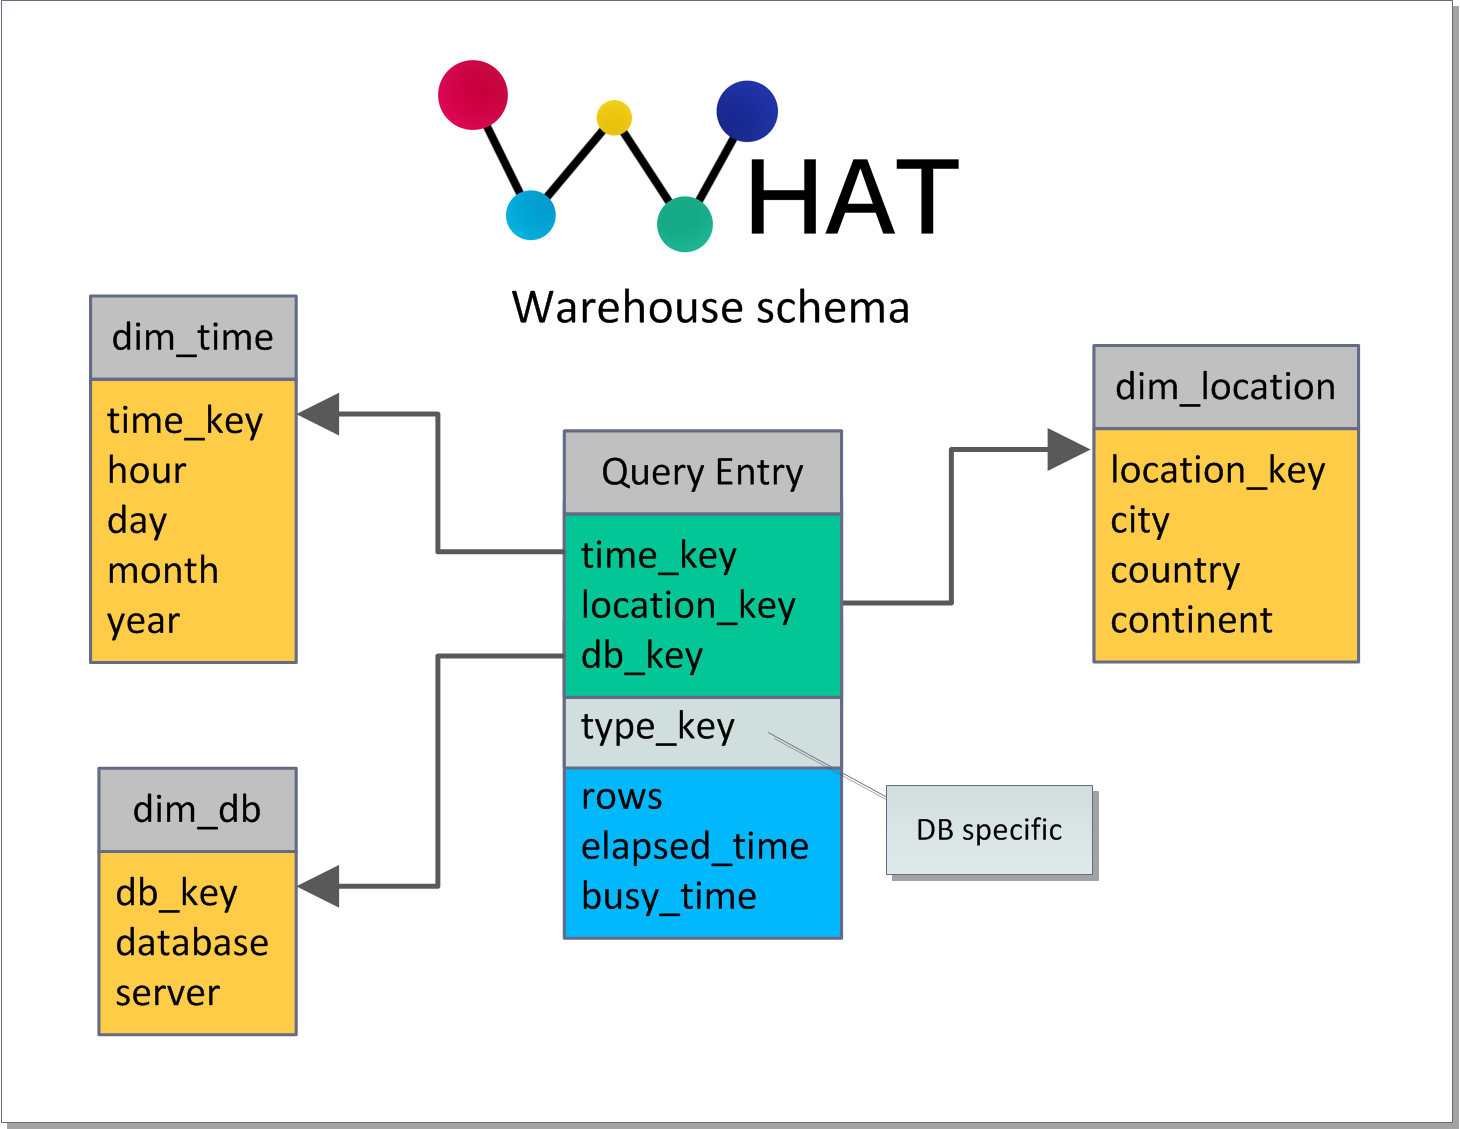
\includegraphics[width=1\linewidth]{Pictures/WHSchema.png}
% or
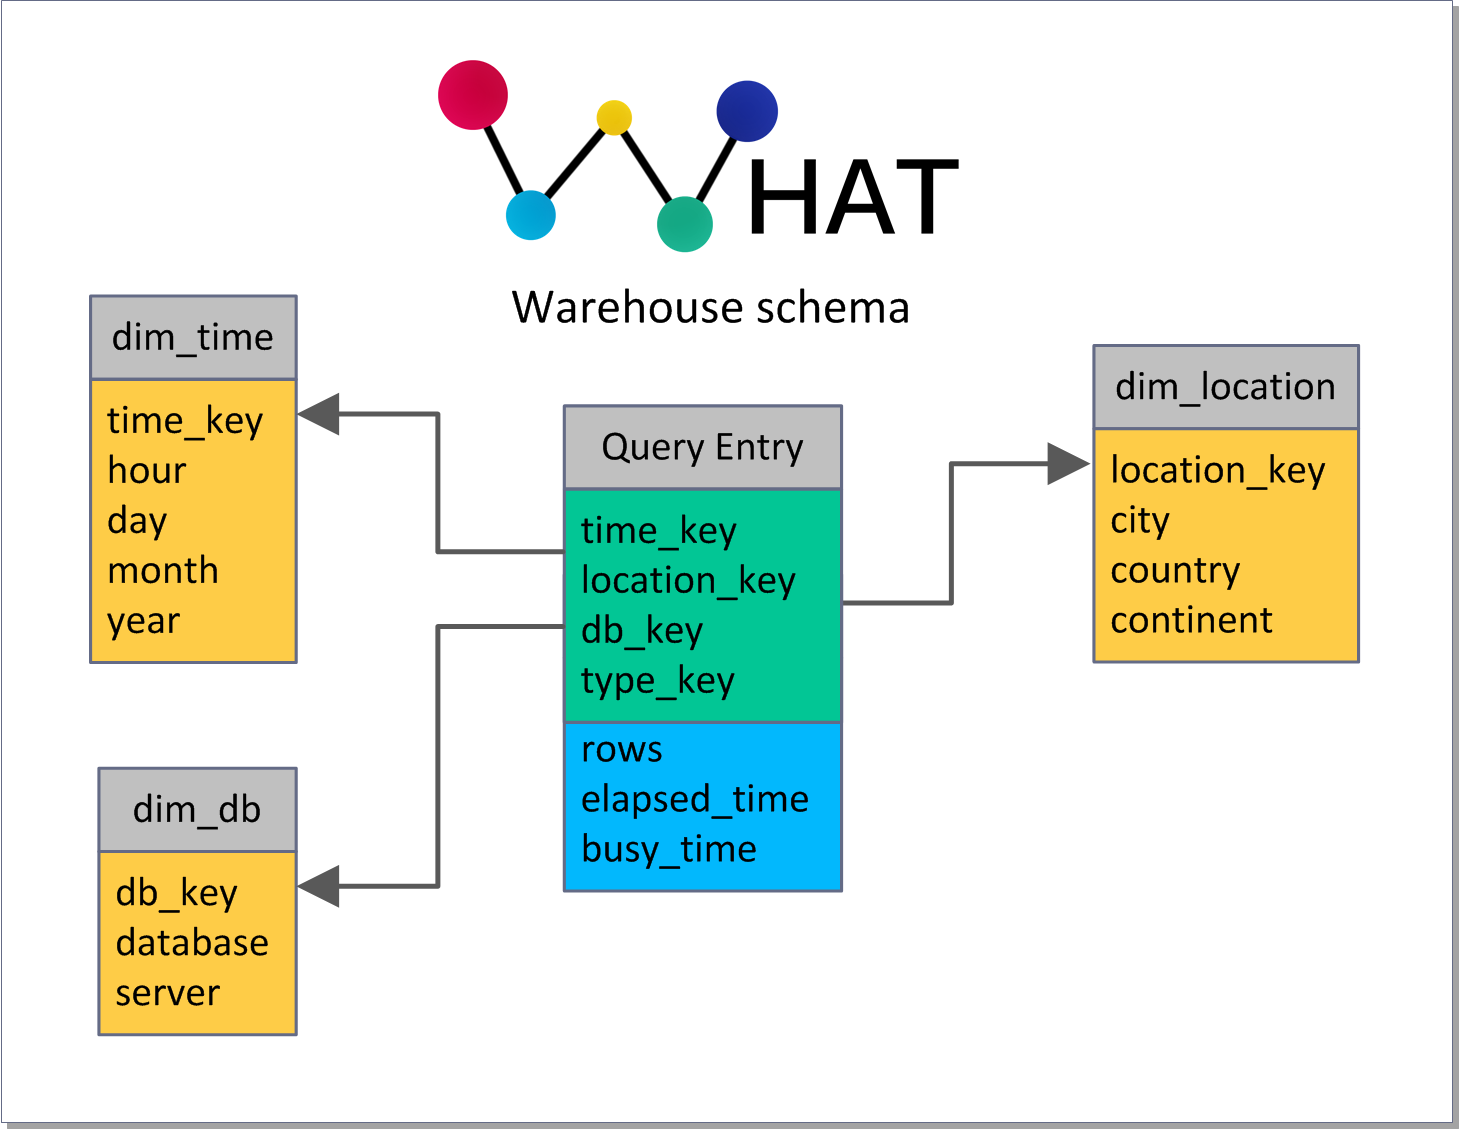
\includegraphics[width=1\linewidth]{Pictures/WHSchema2.png}
\end{center}   


\subsection{Dimension descriptions}
 
\subsection{Measure descriptions}
Some measures may be 
\subsection{Type description}
As Type depends which data base is operated, it may get it's own subsection.

  